\documentclass[reprint, english, nofootinbib]{revtex4-2}

\usepackage{graphicx}
\usepackage{subfig}
\usepackage[colorlinks=true,urlcolor=blue,citecolor=blue]{hyperref}
\usepackage{physics}
\usepackage{amsmath}
\usepackage{amssymb}
\usepackage{amsbsy}
\usepackage{subfig}
\usepackage{blindtext}
\usepackage{tikzducks}
\usepackage{tikz}
\usepackage{pgfplots}
\usepackage{listings}

\graphicspath{{../figs/}}


\begin{document}
\title{Solving partial differential equations with neural networks}
\author{Nicholas Karlsen}
\affiliation{University of Oslo}
\author{Thore Espedal Moe}
\affiliation{University of Oslo}
\date{\today}

\begin{abstract}
    An abstract abstract
\end{abstract}

\maketitle


\section{Introduction}

\section{Theory}
\subsection{The Heat Equation}
\noindent 
In physics, the Heat equation models how the temperature of some material $u\qty(\pmb r, t)$ evolves over time by the partial differential equation (PDE)
\begin{equation}
    \pdv{u}{t} = c^2\nabla^2 u 
\end{equation}
where $c^2$, the thermal diffusivity is a material dependent constant. 
This may be reduced to a one dimensional problem, modelling i.e a thin, insulating wire of length $L$ as
\begin{equation}\label{eqn: 1D heat eqn}
    \pdv{u}{t} = \pdv[2]{u}{x}
\end{equation}
where we have also for simplicity set $c^2 = 1$. We may then solve this analytically with boundary conditions $u\qty(0, t) = u\qty(L,t) = 0$ and initial condition $u(x, 0) = f(x)$.

We start by making the assumption that $u(x, t)$ is separable, giving 
\begin{equation}
    u(x, t) = F(x) \cdot G(t)
\end{equation}
which lets us rewrite Eqn.~\ref{eqn: 1D heat eqn} to the form
\begin{equation}
    F \cdot \pdv{G}{t} = \pdv[2]{F}{x} \cdot G
\end{equation}
which may be expressed as
\begin{equation}
    \frac{\dot G}{G} = \frac{F^{''}}{F} = k
\end{equation}
where $k$ is some constant. We further have that the boundary conditions may only be satisfied for $k <  0$, so we set $k = -\rho^2$ and write
\begin{equation}
    F^{''} + \rho F = 0 \quad \quad \dot G + \rho^2G = 0
\end{equation}
starting with the spatial equation, we have a general solution in the form 
\begin{equation}
    F(x) = c_1 \cos(\rho x) + c_2 \sin(\rho x)
\end{equation}
where $c_1 = 0$ is fixed by $u(0, t) = $. Similarly, $u(L, t) = 0$ imposes the requirement $\sin(\rho x) = 0$ which is satisfied by setting $\rho = n\pi/L$, yielding a discrete spectrum of solutions
\begin{equation}
    F_n(x) = \sin\qty(\frac{n\pi x}{L})
\end{equation}
where we omit the constant $c_1$, which we will include later in $G(t)$. 

We then move on to the temporal part, $G(t)$, which we write as
\begin{equation}
    \dot G = -\rho^2G
\end{equation}
which we immediately recognize as having a general solution
\begin{equation}
    G(t) = c_n e^{-n\pi t / L}
\end{equation}
Thus, $u(x, t)$ is solved by a superposition of the discrete set of eigenfunctions
\begin{equation}
    u_n\qty(x, t) = \sum_{n=1}^{\infty} c_n \sin\qty(\frac{n\pi x}{L}) e^{-n\pi t / L}
\end{equation}
with initial condition
\begin{equation}
    u(x, 0) = \sum_{n=1}^{\infty} c_n \sin\qty(\frac{n\pi x}{L}) = f(x)
\end{equation}
a Fourier series. Thus, the coefficients $c_n$ are determined by the integral
\begin{equation}
    c_n = \frac{2}{L}\int_0^L \dd x \, f(x) \sin\qty(\frac{n\pi x}{L})
\end{equation}
if we set the initial condition $f(x) = \sin(\pi x)$ and fix $L = 1$, we get coefficients
\begin{equation}
    c_n = 2\int_0^1 \dd x \, \sin(\pi x) \sin(n\pi x) = 1
\end{equation}
we thus have an analytical solution for the Heat equation with boundary conditions $u(0, t) = u(L, t) = 0$, $L = 1$, and initial condition $u(x, 0) = \sin(\pi x)$ as
\begin{equation}
    u(x, t) = \sin\qty(\pi x) e^{-\pi t}
\end{equation}
a plot of which for $t \in [0, 1]$ is shown in Fig.~\ref{fig: heat eqn analytic}.
\begin{figure}[h!tb]
    \center
    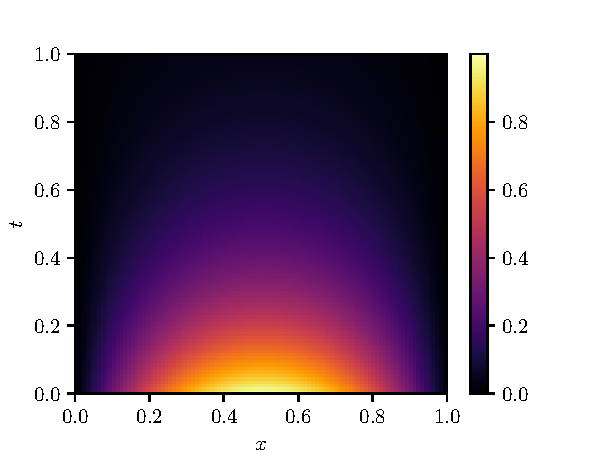
\includegraphics[width=.8\columnwidth]{heat_eqn_analytic.pdf}
    \caption{\label{fig: heat eqn analytic}}
\end{figure}

\subsection{Forward-Euler}


\subsection{Solving ODEs with Neural Networks}
\noindent
In general, a ordinary differential equation (ODE) may be written in the form
\begin{equation}
    F \qty[x, u(x), u'(x), u''(x), \dots, g^{(n)}(x)] = 0
\end{equation}    
where $u(x)$ denotes the solution of the ODE. One may then propose a trial solution $u_t(x,P)$ in the form
\begin{equation}
    u_{t}(x, P) = u_{bc}(x) + u_{nn}(x)N(x, P) 
\end{equation}
where $u_{bc}(x), u_{nn}(x)$ are functions which enforce the boundary conditions of the ODE and $N(x, P)$ is a neural network with independent variables denoted by $P = \{W\},\{\pmb b\}$, the weights and biases in the network respectively.. In order to optimize $N(x, P)$ such that $u_t(x)$ yields a solution of the ODE, we define the cost function by the $L^2$ norm of $F$ as
\begin{equation}
    \mathcal C\qty[u\qty(x)] = \frac{1}{N} \sum_{i=1}^{N}\qty(F\qty[x, u(x_i), u'(x_i), \dots, u^{(n)}(x_i)])^2
\end{equation}
where we have discretized as $x \rightarrow \{x_1, x_2 ,\dots, x_{N}\}$. We can then construct a Feed-Forward Neural network with $L-1$ hidden layers which for each itteration updates the weights and biases of the network wrt. to the current trial solution $u_t(x)$ evaluated with the cost function. See \cite{4155_project_2}


\subsection{Solving the Heat Equation with Neural Networks}
\noindent
We may now using the methods introduced in the previous section design a method to solve the Heat equation using a neural network. We start by re-writing Eqn.~\ref{eqn: 1D heat eqn} to the form
\begin{equation}
    \pdv{u}{t} - \pdv[2]{u}{x} = 0
\end{equation}
which gives rise to the cost function 
\begin{equation}
    \mathcal C\qty[u\qty(x, y)] = \frac{1}{N}\sum_{i=1}^N \qty(\pdv{u}{t} - \pdv[2]{u}{x})^2
\end{equation}
setting the boundary conditions $u(0, t) = u(L, t) = 0$ and initial condition $u(x, 0) = \sin(\pi x)$, we then have a trial solution in the form
\begin{equation}
    u_t(x, t, P) = \qty(1 - t)\sin(\pi x) + x(1 - x)t N(x, t, P)
\end{equation}

\begin{figure}[h!tb]
   \center
   


\tikzset{every picture/.style={line width=0.75pt}} %set default line width to 0.75pt        

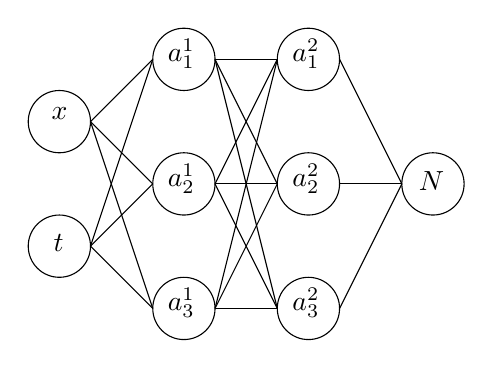
\begin{tikzpicture}[x=0.75pt,y=0.75pt,yscale=-1,xscale=1]
%uncomment if require: \path (0,695); %set diagram left start at 0, and has height of 695

%Shape: Ellipse [id:dp613538016915602] 
\draw   (80,265) .. controls (80,256.72) and (86.72,250) .. (95,250) .. controls (103.28,250) and (110,256.72) .. (110,265) .. controls (110,273.28) and (103.28,280) .. (95,280) .. controls (86.72,280) and (80,273.28) .. (80,265) -- cycle ;
%Shape: Ellipse [id:dp15712636391006307] 
\draw   (80,205) .. controls (80,196.72) and (86.72,190) .. (95,190) .. controls (103.28,190) and (110,196.72) .. (110,205) .. controls (110,213.28) and (103.28,220) .. (95,220) .. controls (86.72,220) and (80,213.28) .. (80,205) -- cycle ;
%Shape: Ellipse [id:dp8164179950038163] 
\draw   (140,175) .. controls (140,166.72) and (146.72,160) .. (155,160) .. controls (163.28,160) and (170,166.72) .. (170,175) .. controls (170,183.28) and (163.28,190) .. (155,190) .. controls (146.72,190) and (140,183.28) .. (140,175) -- cycle ;
%Shape: Ellipse [id:dp47375219812723146] 
\draw   (140,235) .. controls (140,226.72) and (146.72,220) .. (155,220) .. controls (163.28,220) and (170,226.72) .. (170,235) .. controls (170,243.28) and (163.28,250) .. (155,250) .. controls (146.72,250) and (140,243.28) .. (140,235) -- cycle ;
%Shape: Ellipse [id:dp712019427556807] 
\draw   (140,295) .. controls (140,286.72) and (146.72,280) .. (155,280) .. controls (163.28,280) and (170,286.72) .. (170,295) .. controls (170,303.28) and (163.28,310) .. (155,310) .. controls (146.72,310) and (140,303.28) .. (140,295) -- cycle ;
%Straight Lines [id:da6435868346848231] 
\draw    (110,205) -- (140,175) ;
%Straight Lines [id:da08712551076022779] 
\draw    (110,265) -- (140,235) ;
%Straight Lines [id:da18860583656122687] 
\draw    (110,265) -- (140,175) ;
%Straight Lines [id:da267566031093317] 
\draw    (110,265) -- (140,295) ;
%Straight Lines [id:da6453145574577351] 
\draw    (110,205) -- (140,295) ;
%Straight Lines [id:da9129290543985238] 
\draw    (110,205) -- (140,235) ;
%Shape: Ellipse [id:dp31900160827767665] 
\draw   (200,175) .. controls (200,166.72) and (206.72,160) .. (215,160) .. controls (223.28,160) and (230,166.72) .. (230,175) .. controls (230,183.28) and (223.28,190) .. (215,190) .. controls (206.72,190) and (200,183.28) .. (200,175) -- cycle ;
%Shape: Ellipse [id:dp21066050092203037] 
\draw   (260,235) .. controls (260,226.72) and (266.72,220) .. (275,220) .. controls (283.28,220) and (290,226.72) .. (290,235) .. controls (290,243.28) and (283.28,250) .. (275,250) .. controls (266.72,250) and (260,243.28) .. (260,235) -- cycle ;
%Shape: Ellipse [id:dp8190479437064692] 
\draw   (200,235) .. controls (200,226.72) and (206.72,220) .. (215,220) .. controls (223.28,220) and (230,226.72) .. (230,235) .. controls (230,243.28) and (223.28,250) .. (215,250) .. controls (206.72,250) and (200,243.28) .. (200,235) -- cycle ;
%Shape: Ellipse [id:dp9436580210127415] 
\draw   (200,295) .. controls (200,286.72) and (206.72,280) .. (215,280) .. controls (223.28,280) and (230,286.72) .. (230,295) .. controls (230,303.28) and (223.28,310) .. (215,310) .. controls (206.72,310) and (200,303.28) .. (200,295) -- cycle ;
%Straight Lines [id:da5770582110402913] 
\draw    (170,175) -- (200,175) ;
%Straight Lines [id:da378598346323751] 
\draw    (170,175) -- (200,235) ;
%Straight Lines [id:da045787154766960936] 
\draw    (170,175) -- (200,295) ;
%Straight Lines [id:da10461814863080832] 
\draw    (170,295) -- (200,175) ;
%Straight Lines [id:da18820240172871194] 
\draw    (170,295) -- (200,235) ;
%Straight Lines [id:da7563044436713307] 
\draw    (170,295) -- (200,295) ;
%Straight Lines [id:da9591828994155338] 
\draw    (170,235) -- (200,295) ;
%Straight Lines [id:da039530432138651816] 
\draw    (170,235) -- (200,235) ;
%Straight Lines [id:da03185694587768484] 
\draw    (170,235) -- (200,175) ;
%Straight Lines [id:da6835990243055697] 
\draw    (230,235) -- (260,235) ;
%Straight Lines [id:da4490575310089562] 
\draw    (230,295) -- (260,235) ;
%Straight Lines [id:da36571324995783205] 
\draw    (230,175) -- (260,235) ;

% Text Node
\draw (91,258) node [anchor=north west][inner sep=0.75pt]    {$t$};
% Text Node
\draw (90,197) node [anchor=north west][inner sep=0.75pt]    {$x$};
% Text Node
\draw (146,164) node [anchor=north west][inner sep=0.75pt]    {$a^{1}_{1}$};
% Text Node
\draw (146,224) node [anchor=north west][inner sep=0.75pt]    {$a^{1}_{2}$};
% Text Node
\draw (146,284) node [anchor=north west][inner sep=0.75pt]    {$a^{1}_{3}$};
% Text Node
\draw (206,164) node [anchor=north west][inner sep=0.75pt]    {$a^{2}_{1}$};
% Text Node
\draw (267,228) node [anchor=north west][inner sep=0.75pt]    {$N$};
% Text Node
\draw (206,224) node [anchor=north west][inner sep=0.75pt]    {$a^{2}_{2}$};
% Text Node
\draw (206,284) node [anchor=north west][inner sep=0.75pt]    {$a^{2}_{3}$};


\end{tikzpicture}
 
   \caption{Possible network structure of a Feed-Forward network with input $(x,t)$ and 2 hidden layers each with 3 neurons with activations denoted as $a^l_j$} and a single output $N$.
\end{figure}


\section{Results \& Discussion}

\section{Conclusion}

\onecolumngrid
\bibliography{bibfile}
\twocolumngrid

\end{document}